\documentclass[]{article}

\usepackage{graphicx}
\usepackage{float}
\usepackage[a4paper,top=2.5cm,bottom=2.5cm,left=2.5cm,right=2cm]{geometry}
\usepackage{subcaption}
\usepackage[table,xcdraw]{xcolor}
\usepackage{makecell}
\usepackage{tabularx}
\usepackage{enumitem}

\setlength{\tabcolsep}{13pt}
\renewcommand{\arraystretch}{2.3}

\title{ RASD \\
	\begin{large} 
		Software Engineering 2
	\end{large}}

\author{Antonio Ercolani - 10621728\\Vittorio Fabris - 10562731\\Riccardo Nannini - 10626268}
\date{Academic year 2020/2021}


\begin{document}
	\pagenumbering{gobble}
	
	\maketitle
	\begin{paragraph}
		\newline
	\end{paragraph}

	\newpage
	\pagenumbering{arabic}	


	\tableofcontents
	
	\newpage
	
	
	\section{Introduction}
	
	\subsection{Purpose}
	
	The \textit{Requirement Analysis and Specification Document} (RASD) is a standardized document used by software engineers to communicate the most important aspects of a system to be developed to the project stakeholders. The RASD represents the starting point of the so called “waterfall life-cycle” of a software system, therefore it’s easy to understand how delicate and strategical is the role it performs. Programmers, testers, designers and everyone involved in the development will refer to this paper and a mistake could potentially cost thousand hours of additional work. 
	\smallskip
	\\
	What we said so far is the purpose of this document. This specific RASD is about an application that tries to face the crowding of supermarkets during the coronavirus emergency. In the following section we are going to explain the scope of that software system.

	\subsection{Scope}
	
		\begin{paragraph}
			\newline
				The scope of the software is to give the users the possibility to line up to enter and shop into a grocery stores.\\
				The stores that have registered to this service generate and distribute tickets to line people correctly, letting them do the shopping only if the QR-code scanned on their ticket is valid.\\
				CLup offers different kind of functionalities and features:\\
	
			\begin{itemize}
			\item \textbf{Basic:}
				The user can line up in different ways: through a physical ticket taken outside the store, or through the application, that is implemented in a way such that people of every age can use. \\
				If there are already too many people queuing outside the shop, the software doesn’t allow to distribute new physical tickets. \\
				The software can integrate the information derived  from the two sources, virtual and physical bookings, so that overcrowding is avoided in the neighborhood of the store and thanks to the QR ticket validations, store managers can monitor entrances. \\
				When the user leaves the store he must show his ticket to the QR-reader again, so that the system can know it and let the queue proceed, with another customer enter the shop.\\

			\item \textbf{Feature 1:}
				Users that line up from home concede the system to see where they are, using the GPS position of their device to identify their zone. In this way only nearby grocery stores are shown to the user.\\
				What’s more, these category of users can book a visit at a specific time, if there is a free spot in the schedule organized by the system, otherwise other arrival times or grocery stores are proposed to the user.\\
				The system, knowing the position of the user, his distance from the store and the vehicle that he has chosen to use to reach it, will provide him a notification that in a certain moment he should leave to arrive on time at the grocery store. If the user arrives late, the system can reschedule a booking for him, always considering to avoid overcrowding and the time preferences of the customer, inserting him into the line again.\\

			\item  \textbf{Feature 2:}
				Because the system needs to balance in the best way possible the number of people inside the store, the user that books online his visit is also asked which kind of products he’s going to buy. In this way the system can manage people along the store’s aisles, reducing the possible interaction and proximity of customers, distributing their access into the shop in different times if it is necessary.  \\

			\item  \textbf{Feature 3:}
				When the grocery store registers to the service, it can decide if he wants to save the information about the preferences of customers about the products they buy. In fact, as explained in the previous feature, the user lets the system know what he intends to buy. The grocery store could use these preferences in order to manage a plan for the refill of its shelves and always be ready to satisfy the needs of  its customers, avoiding the risk of not having some products to sell, but ordering them from their providers in advance.

			\end{itemize}
			
	
		\end{paragraph}
	
		\subsubsection{World phenomena}

			\begin{tabular}{|c|l|}
				\hline
				\rowcolor[HTML]{DCDCDC} 
				\textbf{WP1} & The customer arrives to the store \\ \hline
				\textbf{WP2} & The customer shops in the store \\ \hline
				\rowcolor[HTML]{DCDCDC} 
				\textbf{WP3} & The customer waits outside the store \\ \hline
			\end{tabular}
			
		\subsubsection{Shared phenomena}
		
			Controlled by the \textbf{machine}\newline\newline
					\begin{tabular}{|c|l|}
						\hline
						\rowcolor[HTML]{DCDCDC} 
						\textbf{SP1} & The customer is notified that his turn is coming \\ \hline
						\textbf{SP2} & The store generates and sends a ticket to the user (?) \\ \hline
					\end{tabular} \newline\newline\newline
			Controlled by the \textbf{world}\newline\newline
					\begin{tabular}{|c|l|}
						\hline
						\rowcolor[HTML]{DCDCDC} 
						\textbf{SP3} & The customer enters the store scanning his QR code \\ \hline
						\textbf{SP4} & The customer reserves a place in the queue of a given store using the application \\ \hline
						\rowcolor[HTML]{DCDCDC} 
						\textbf{SP5} & \makecell[l]{The customer reserves a place in the queue of a given store using the ticket totem \\outside the store}\\ \hline
						\textbf{SP6} & The customer books a visit to the store \\ \hline
						\rowcolor[HTML]{DCDCDC} 
						\textbf{SP7} & The customer leaves the store \\ \hline
						\textbf{SP8} & The store receives a request to join its queue \\ \hline
					\end{tabular}
					
		
		\subsubsection{Goals}
		
		\begin{tabular}{|c|l|}
						\hline
						\rowcolor[HTML]{DCDCDC} 
						\textbf{G1} & \makecell[l]{At any time the number of people in the store must not be higher than the store limit or \\ the limit is passed but the customers are expected to be in different areas of the store} \\ \hline
						\textbf{G2} & The physical queue of people outside the store is reduced \\ \hline
						\rowcolor[HTML]{DCDCDC} 
						\textbf{G3} & Allow users to "line up" for a store from home \\ \hline	 
						\textbf{G4} & Allow users to book a visit to a store \\ \hline
						\rowcolor[HTML]{DCDCDC}
						\textbf{G5} & Balance the number of people between different store or timeframes with suggestions \\ \hline		
						\textbf{G6} & Allow the store to monitor entries \\ \hline	
						\rowcolor[HTML]{DCDCDC} 
						\textbf{G7} & Collects information in order to build statistics and infer mean datas \\ \hline					
					\end{tabular}
\newline\newline

	\subsection{Definitions, Acronyms, Abbreviations}
	
	In this section we explain the meaning of some technical terms used in the document.
	\medskip
	\\
	\begin{tabular}{|c|l|}
		\hline
		\rowcolor[HTML]{DCDCDC} 
		\textbf{QR CODE} & \makecell[l]{A \textit{Quick Response code} is a kind of bar-code, readable by machines to retrieve information} \\ \hline
		\textbf{ASAP} & \makecell[l]{An \textit{As Soon As Possible} preference indicates that the customer wants to line up\\immediately, without booking a visit at a specific time to enter the store} \\ \hline
		\rowcolor[HTML]{DCDCDC} 
		\textbf{UML} & \makecell[l]{The \textit{Unified Modeling Language} is a modeling language used to describe the design \\of a software system} \\ \hline
	\end{tabular}
	
	
	
	
	\subsection{Revision history}	
	\subsection{Reference Documents}
	
	\subsection{Document Structure}
	
	This RASD document is structured over 6 main chapters, described below.
	
	\paragraph{Chapter 1} starts with a brief description of the purpose of this document. Then the focus moves on the involved software system, for which is given an overall description of the goals, scope and related phenomena. The chapter ends with secondary sections about the description of technical terms and the history of this RASD document.
	
	\paragraph{Chapter 2} let the reader to better understand the "world" of the analyzed software system. It begins with a UML and then other kind of diagrams that explain how the application interact with the environment around it. The following sections are about the requirements the system must satisfy, also with a focus on the specific users needs. Finally, in the last section, we list the domain assumption we did.
	
	\paragraph{Chapter 3} goes deep into the topics described in the previous chapter.
	Begins with the description of the user interface and continue with use cases and sequence diagrams to show how the system behaves in different situations, in respect to the application requirements. Then you will find sections on other system constraints on performance and design. The chapter ends with few words on non-functional requirements.
	
	\paragraph{Chapter 4} tries to describe the main aspects of the software system we have seen so far with an alloy model.
	
	\paragraph{Chapters 5 and 6} contain, respectively, an outline of the effort spent in the project by each team mates and the document references.
	
	\newpage
	\section{Overall description}
	
		\subsection{Product perspective}
		The CLup system is designed as a complitely new software application. The user side of the software is intended to be used as a mobile application while the store managers are going to interface with the software through a web interface. \newline
		In order to estimate the time needed for the user to reach the store, the application needs to interface with the smartphone's localization system and needs the user to indicate the type of transportation that he is going to use. \newline
		The system will handle client that are not using the application with tickets provided by a ticket totem located outside the store. This machine will act as an interface to the software application. \newline
		Customers using CLup are going to be notified when their turn is coming in order to approach the store while those with a ticket outside the store will monitor a screen extern to the shop in order to know when it's their turn to enter. \newline
		In order to access the store, every customer is required to scan their QR code (either from the application or from the physical ticket) when entering and exiting the store: in both cases the system will activate an automatic door. \newline
		On the other side of the system, store managers are going to be able to monitor and manage the queue of their store as well as programmed visits. \newline
		The below class diagram models the application domain in order to give an overlook on the enviroment where the application is going to work.
		
		\begin{figure}[htp]
			\centering
			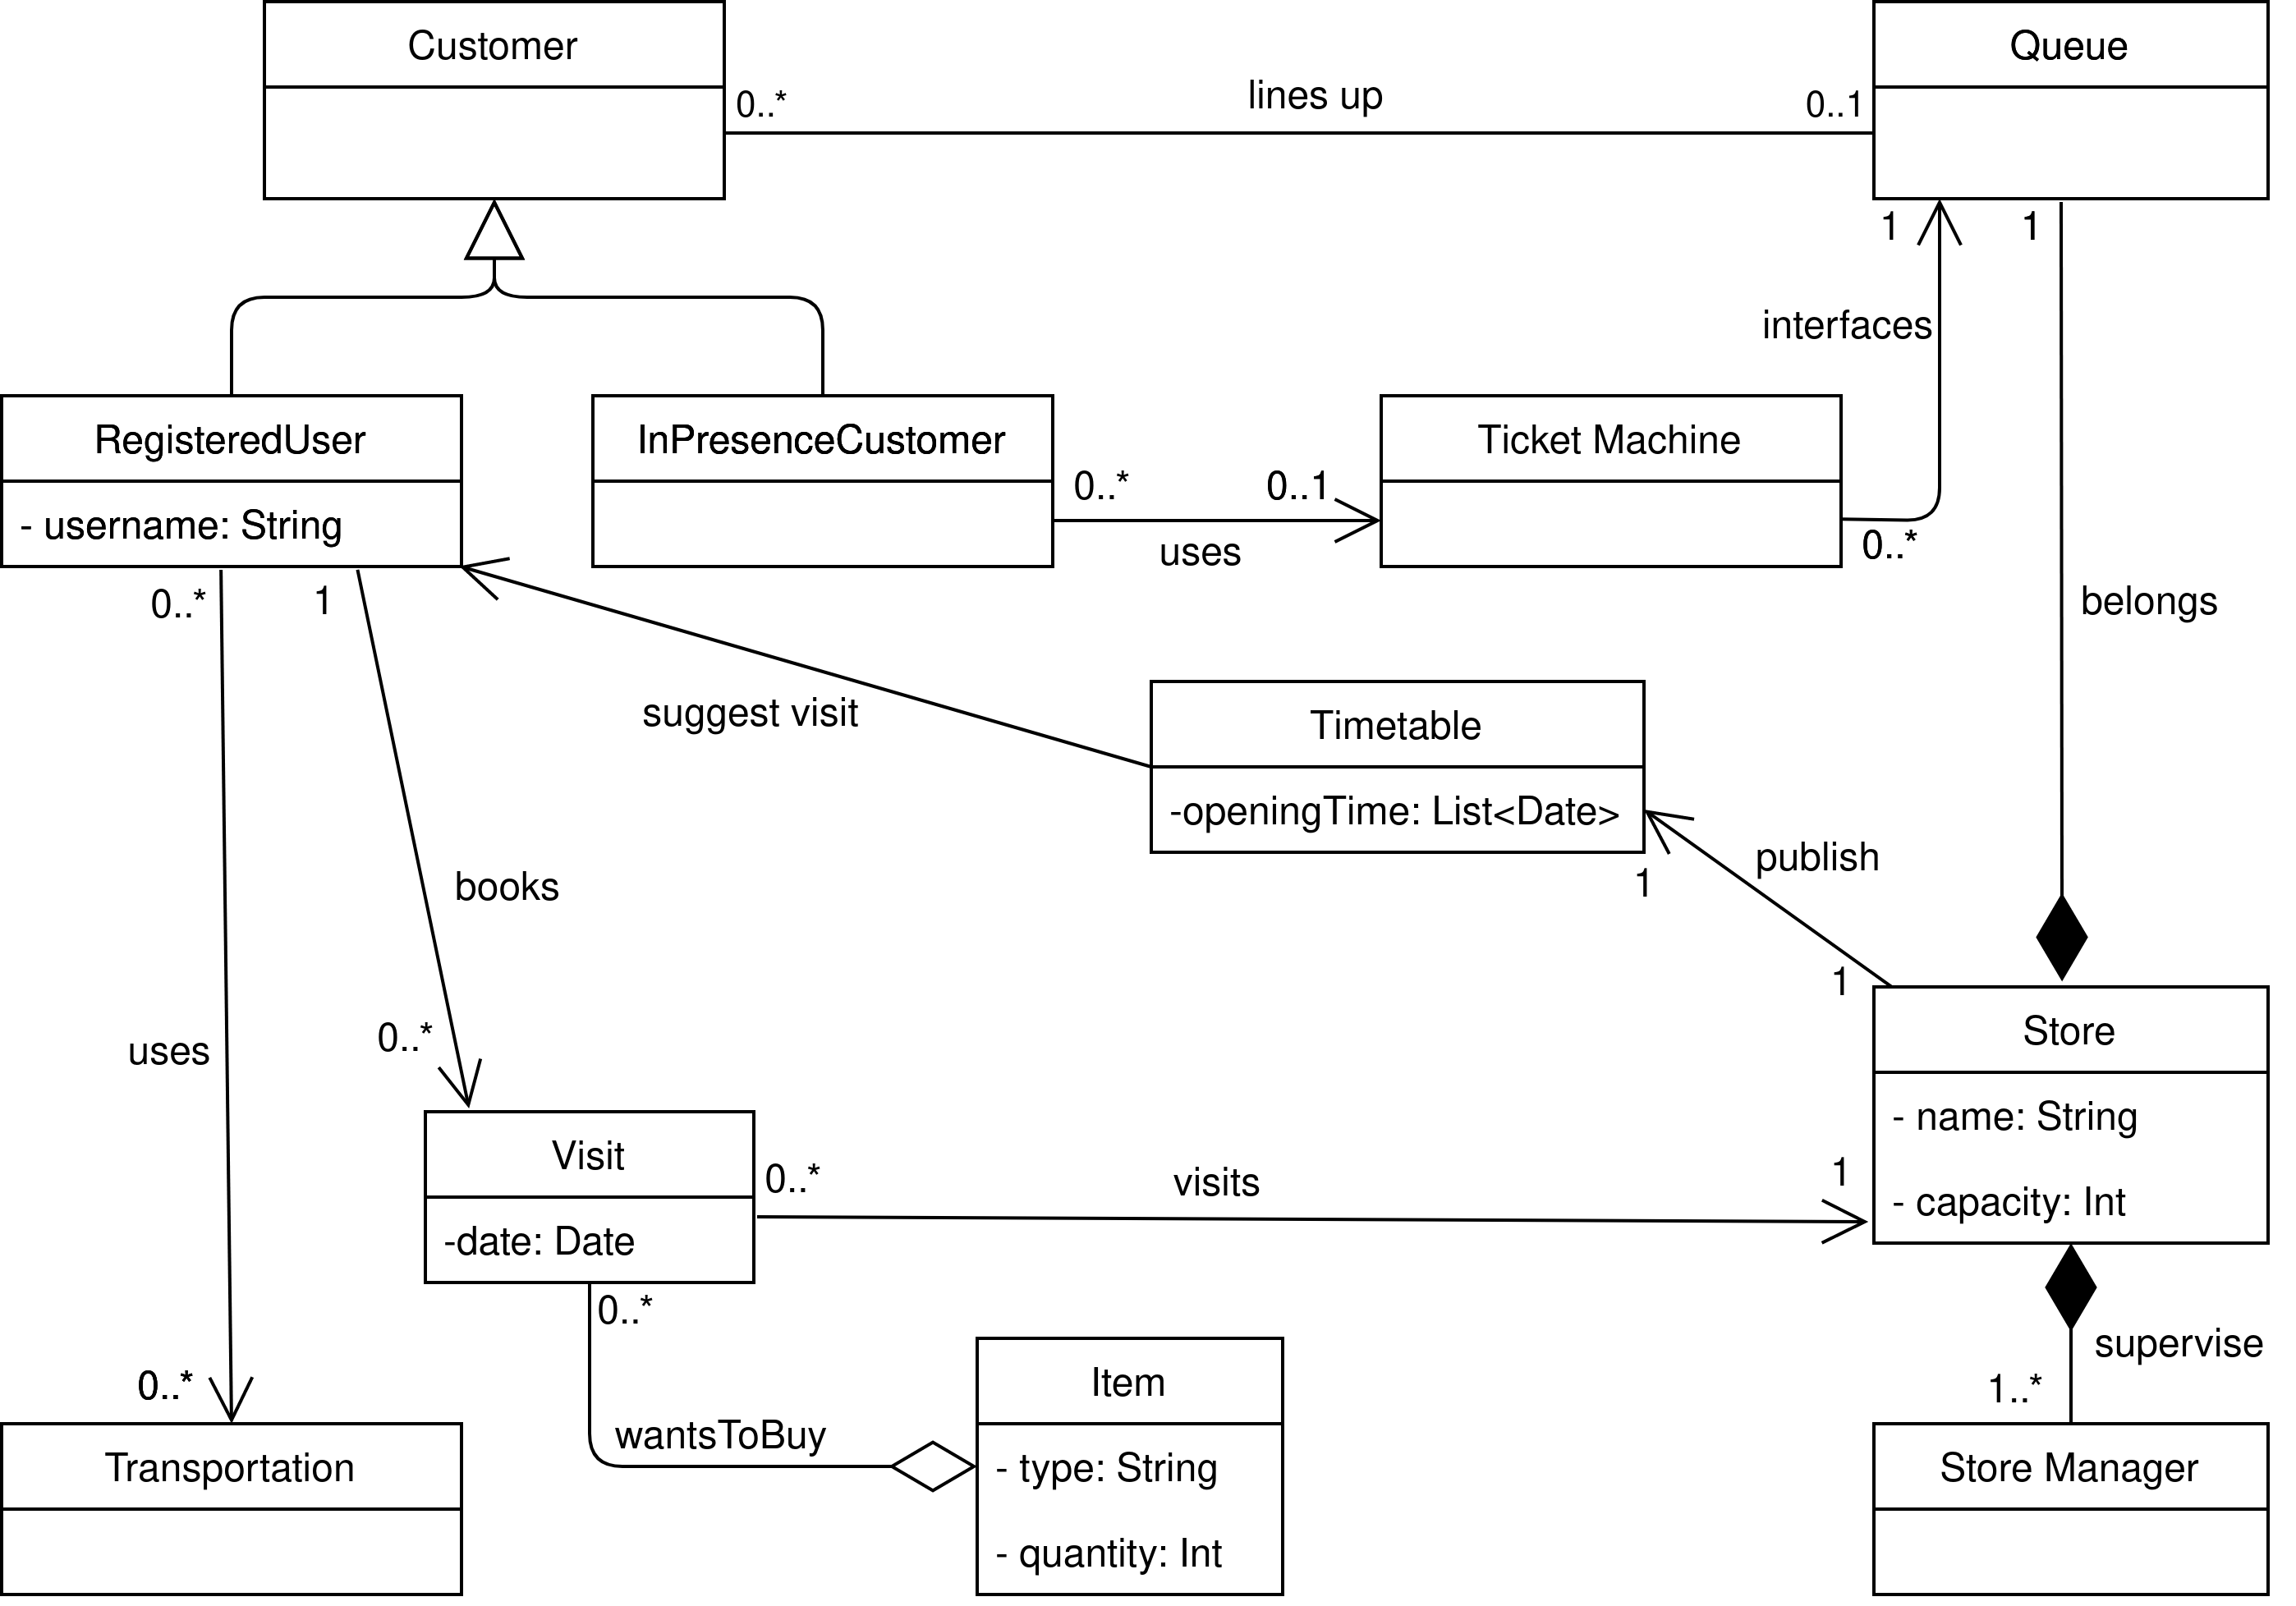
\includegraphics[scale=0.5]{UML_class_diagram.png}
			\caption{Class diagram}
			\label{fig:class_diagram}
		\end{figure}
		
	\textbf{}\\
		\subsection{State Diagrams}
		
		\textbf{}\\ \newline
		In this section we want to show the evolution over time of the states of the application and the behavior of the user interacting with the app and the environment. 
The state diagrams below better explain the progress of the system.\\
		
		\textbf{}\\ \newline
		
		\begin{figure}[H]
			\centering
			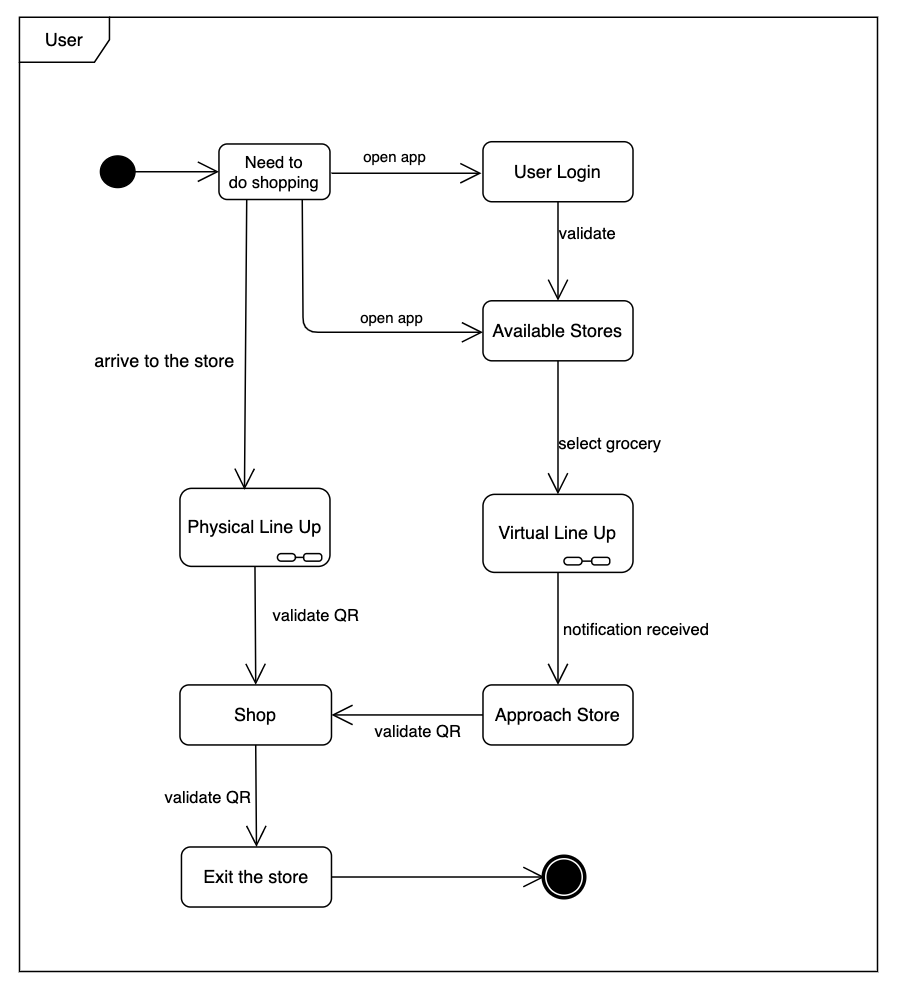
\includegraphics[scale=0.5]{User_statediagram.png}
			\caption{User State Diagram}
			\label{fig:state_diagram1}
		\end{figure}
		
		
		In the first state diagram (Figure \ref{fig:state_diagram1}) it’s shown how the user interacts with the environment and the system when he needs to do shopping. He interacts with the system lining up to a store in a virtual way using the mobile or web application, or queuing physically at the store he wants to visit.
What’s more, to enter the store, he needs to show the QR-code, and then he has to do the same when he exits, so that the queue can proceed. \\

		\textbf{}\\ \newpage

		\begin{figure}[H]
			\centering
			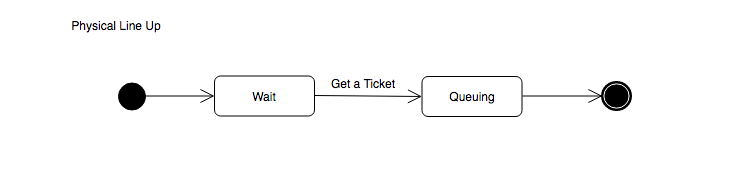
\includegraphics[width=\linewidth]{PhysicalLineUp_statediagram.png}
			\caption{Physical Line Up State Diagram}
			\label{fig:state_diagram2}
		\end{figure}
		
		
		In this second state diagram (Figure \ref{fig:state_diagram2}) it’s better explained the physical line up of the user, that waits and directly gets a ticket from the totem nearby the store. The user then waits for his turn to enter and do the shopping.\\
		
		\textbf{}\\ \newline
		\textbf{}\\ \newline
		
		\begin{figure}[H]
			\centering
			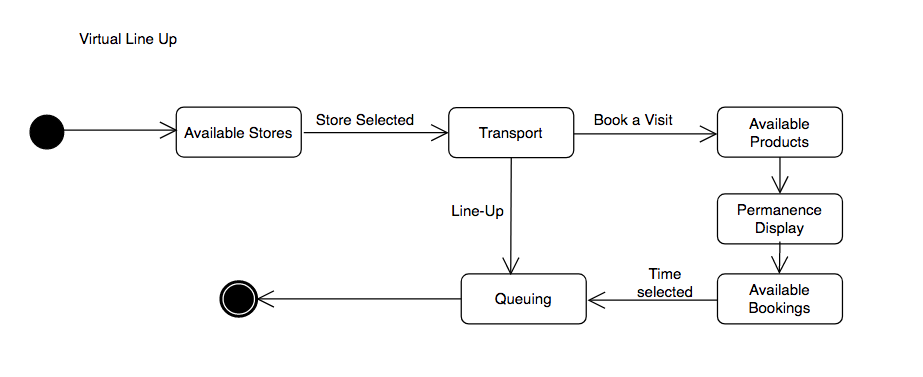
\includegraphics[width=\linewidth]{VirtualLineUp_statediagram.png}
			\caption{Virtual Line Up State Diagram}
			\label{fig:state_diagram3}
		\end{figure}
		
		Here (Figure \ref{fig:state_diagram3})  are shown the steps to go through the virtual line up of the user, that has to face some intermediate steps before gaining the possibility to line up to the store. When the store has been selected, the user needs to indicate the transportation he will use to reach the store. Then, if he doesn't want to line up immediately but wants to book a visit, he will see the available products that he can buy and will have to choose which one of them he wants to buy, so that the system can collect his preferences. Then the user is asked to indicate his permanence into the store, in order to better manage the queue and the next available spots in the timeline. \\
		

\newpage

\subsection{Product functions}

In this section are analyzed the main functionalities that the CLup software system must ensure. Goals and requirements are many and they are all connected with each other, therefore, below you will find the description of two "macro-functionalities" that try to group most of them. Said that, in order to go deeply in every system capability, the reader should supplement this section with the next chapter - "Specific requirements".
\bigskip
\\
\begin{large}
	\textbf{Queue management}
\end{large}
\smallskip
\\
The core function. As the name suggest, the system is able to manage the stores entering queue, that are becoming longer and "dangerous" in the time of coronavirus. This is done with a combination of two sub-functionalities: 

\begin{itemize}
	\renewcommand{\labelitemi}{$-$}
	\item \textbf{Line up from home} - allow users to reserve their place in the queue without having to reach the store, they just need to access the application and choose a grocery. To this simple user action corresponds an important data elaboration made by the system, to ensure another important functionality: \textbf{alert the costumer when his turn comes}. In fact the system must take into account different factors to alert the user in the right moment:
	\begin{itemize}
		\renewcommand{\labelitemi}{$-$}
		\item The distance between the user home and the selected store;
		\item The means of transport by which the costumer intend to reach the store,
		\item How much time take people before the user in the queue to enter the store.
	\end{itemize} 
	Once the system has collected all the information, it can compute the right amount of time needed by the costumer to reach the store in the right moment he have to enter in.
	\item \textbf{Line up physically} - the system must give the possibility to line up physically. Therefore, when costumers reserve their place directly at the store the system must collect also this data. Obviously, for them there is no need to compute any kind of time to enter in the store because they wait for their turn right outside.
\end{itemize}	
\begin{large}
	\textbf{Booking visits}
\end{large}
\smallskip
\\
The second macro-functionality is the possibility of \textbf{booking a visit} to a registered store. On the costumers side, this functionality could be similar to the previous one but the main difference lies on the side of the stores. In fact the information that the costumers provide to the system during the booking is essential to the next presented feature.
\begin{itemize}
	\renewcommand{\labelitemi}{$-$}
	\item \textbf{Increase the capacity of the stores} - the system should allow more people in the stores than the standard number. This is made possible by asking to the costumer who book a visit the categories of items he's intended to buy, therefore the system can infer which sectors of the store he's going to occupy. These information are exploited by the system to maximize the capacity of the stores, respecting the social distancing imposed by the coronavirus emergency rules.
\end{itemize}
The second feature of the list is also directly linked to the "booking".
\begin{itemize}
	\renewcommand{\labelitemi}{$-$}
	\item \textbf{Balance out the number of people in the store} - the system should be able to balance out the number of people in the different registered stores. This is done by suggesting people alternative time slots or different stores when they are booking a visit.
\end{itemize}
\bigskip
\begin{large}
	\textbf{General store management}
\end{large}
\smallskip
\\
The last functionality allows store managers to visualize all the collected information about the store. For example, store managers can check how many customers are queuing outside the store, how many of them are doing shopping in a given moment and the booked visits of the following days.  

\newpage

\subsection{User characteristics}
The CLup software system involves category of users:
\begin{itemize}
	\renewcommand{\labelitemi}{$-$}
	\item \textbf{Costumers} - are client of the registered stores that want to take advantage of the CLup features. They are interested in the possibility of "line up" from home and in "booking visits", that encourage them to continue go shopping, despite the problem caused by the emergency.
	
	\item \textbf{"Stores"} - these users are represented by the stores that want to take advantage of the CLup services. They have to follow a registration procedure to be added to the available stores of the system. 
	\\Besides exploit the "remote lining up" function that mainly face social distancing, they are interested in other features such as "increase the capacity of the stores" and "balance out the number of people in the store". In fact exploiting them they could are able to keep profits high, despite the coronavirus emergency. 		
\end{itemize}


	
	\section{Specific requirements}
	
		\subsection{External Interface Requirements}
			\subsubsection{User Interfaces}
			TODO UI TELEFONO + UI TICKET TOTEM
			\subsubsection{Hardware Interfaces}
			The system requires different external hardware components in order to work. \newline
			An \textbf{automatic door} needs to be present both in the entrance and the exit of the store. It's necessary in order to effectively regulate and monitor the flow of customers: the doors won't unlock unless the client specific QR Code is scannerized and accepted. \newline
			A \textbf{QR Code scanner} is required in correspondence of the automatic doors for the reason given above. \newline
			At least one \textbf{ticket totem} is needed in order to hand out tickets for customers not using the app. \newline
			In the end, one or more \textbf{monitors} are needed outside the store to let customers know when their turn has come. \newline \newline
			In addition to this, the  two type of actors require different hardware component in order to interact with the system. \newline
			Users need a smartphone with a localization system (tipically GPS), while store managers can access and monitor the system via computer.
			\subsubsection{Software Interfaces}
			The system needs an external software component to handle QR code generation and recognition. \newline (Altro da mettere qui? Non mi viene in mente niente)
			\subsubsection{Communications Interfaces}
			The various actors connect to CLup using an internet connection. \newline
			Hardware components such as automatic doors, ticket totem and QR code scanner interface with the system via IP based protocols.
		\subsection{Scenarios}
		
		\subsubsection{Scenario 1: User lines up from home}
		Antonio is a young engineering student. As known, engineering requires a lot of effort and dedication in order to keep the pace of the various courses. He does not want to waste time in the queues outside groceries shop that became common in the pandemic times. Luckly he knows the CLup service and decides to line up for his favorite store from home. \newline He inserts the type of transportation he is going to use in order to reach the store and joins the virtual queue while he can keep studying safely at home. Once his turn is about to come, he receives a notification from the application right on his smartphone and leaves the house
		
		\subsubsection{Scenario 2: Customer physically lines up}
		Maria is an old lady living alone in his apartment in Milan. She does not own a smartphone nor has plan to buy one in the future: she is okay with her old style house phone. \newline Maria goes weekly to the grocery shop: she directs herself to the ticket machine, retrieves a ticket and safely waits outside the store that his turn is called on the monitor. Once it is arrived, she simply scans her ticket's QR code and access the store.
		
		\subsubsection{Scenario 3: User books a visit}
		Elena is a very busy mother of two. She has very limited time frames where she can shop in a grocery store and not miss other appointments in her schedule. \newline
		Since Elena got to know CLup she loved the service of booking a future visit to a store. She just selects her store and favourite time slot, inserts a few data like estimated shopping time etc. and the magic is done. No more time spent outside the shop and appointment delayed.\newline
		Once the selected day of the visit is arrived, she will receive a notification indicating that she should start to approach the store.
		
		\subsubsection{Scenario 4: User arrives late}
		Riccardo, an enthusiastic user of CLup, received a notification from the system inviting him to reach the store where he previously lined up with the software. \newline
		However, a car accident blocked the road and he finds himself complitely stuck in the traffic. He will eventually reach the store with a big delay and find out that his ticket is expired. \newline He then decides to take another ticket from the ticket machine and wait for his turn.
		
		\subsubsection{Scenario 5: Store manager admints more people in the store}
		Vittorio, the store manager of a grocery store that adopted CLup, is monitoring the situation of the store through the software interface. \newline
		He receives a notification from the sytem indicating that, given the calculation of the software, there are the right conditions to admit more people and momentarily exceed the store limit. \newline
		He consults his guide lines and decides to go on with the operation: he inserts the required data and confirms his choice. \newline
		Shortly after the selected number of clients enter the store.
		
		\subsection{Functional requirements}
		
			\subsubsection{Use Cases}
		
			\begin{paragraph}
			\newline
			\begin{enumerate}
				
			\item{\textbf{Costumer sign up}}
			\medskip
			\\ \\
			\begin{tabular}{|c|l|}
				\hline
				\textbf{Name} & \makecell[l]{Costumer sign up} \\ \hline
				\textbf{Actor} & \makecell[l]{Costumer} \\ \hline
				\textbf{Entry Conditions} & 
				\begin{minipage}[t]{10cm}
					\setlist[enumerate]{label={\arabic*.}, ref={\arabic*}}
					\begin{enumerate}
						\item The costumer has already opened the application that sent him to the “sign in/up” screen
						\item The customer has not a CLup own account \\
					\end{enumerate}
				\end{minipage}
				\\ \hline
				\textbf{Events Flow} & 
				\begin{minipage}[t]{10cm}
					\setlist[enumerate]{label={\arabic*.}, ref={\arabic*}}
					\begin{enumerate}
						\item The costumer clicks the “Create new account” button
						\item The costumer fills the registration form 
						\item The costumer checks the filled form fields and confirms them
						\item The system checks if the provided data are correct and creates the account, storing the user data \\
					\end{enumerate}
				\end{minipage}
				\\ \hline
				\textbf{Exit Conditions} & \makecell[l]{The costumer account is successfully created.} \\ \hline
				\textbf{Exceptions} & 
				\begin{minipage}[t]{10cm}
					The system can detect problems in the submitted registration form (fields filled a in wrong way or even left empty). If it happen, the system notifies it to the user and offer the possibly to re-fill it \\
				\end{minipage}  \\ \hline
			\end{tabular}
			\newpage
			
			
			
			
			\item{\textbf{Store registration}}
			\medskip
			\\ \\
			\begin{tabular}{|c|l|}
				\hline
				\textbf{Name} & \makecell[l]{Store registration} \\ \hline
				\textbf{Actor} & \makecell[l]{Store manager} \\ \hline
				\textbf{Entry Conditions} & 
				\begin{minipage}[t]{10cm}
					\setlist[enumerate]{label={\arabic*.}, ref={\arabic*}}
					\begin{enumerate}
						\item The store manager has already opened the application that sent him to the “sign in/up” screen
						\item The store is not registered yet \\
					\end{enumerate}
				\end{minipage}
				\\ \hline
				\textbf{Events Flow} & 
				\begin{minipage}[t]{10cm}
					\setlist[enumerate]{label={\arabic*.}, ref={\arabic*}}
					\begin{enumerate}
						\item The store manager clicks the “Store registration” button starting the registration procedure 
						\item The manager fills the registration form with the store information and submits it to the system 
						\item The system checks if the mandatory fields are correctly filled 
						\item The system continues the store registration procedure checking:
							\setlist[enumerate]{label={\alph*.}}
							\begin{enumerate}
								\item The validity of the information provided by the manager	
								\item If the store is able to satisfy all the CLup hardware requirements
							\end{enumerate}
						\item The  system completes the store registration storing the collected data \\
					\end{enumerate}
				\end{minipage}
				\\ \hline
				\textbf{Exit Conditions} & 
				\makecell[l]{The store is successfully registrated} \\ \hline
				\textbf{Exceptions} & 
				\begin{minipage}[t]{10cm}
					\setlist[enumerate]{label={\arabic*.}, ref={\arabic*}}
					\begin{enumerate}
						\item The system can detect problems in the filled registration form (fields filled a in wrong way or even left empy) and offer the possibly to re-fill it
						\item The system could discover that the information provided by the system manager are not valid. In this case the registration procedure must be restarted. 
						\item The store could not be able to satisfy the hardware requirements, therefore the system doesn’t allow that store to register in the CLup system
						\\
					\end{enumerate}
				\end{minipage}
				\\ \hline
			\end{tabular}
		
		
		
			\newpage
			\item{\textbf{Costumer sign in}}
			\medskip
			\\ \\
			\begin{tabular}{|c|l|}
				\hline
				\textbf{Name} & \makecell[l]{Costumer sign in} \\ \hline
				\textbf{Actor} & \makecell[l]{Costumer} \\ \hline
				\textbf{Entry Conditions} & 
				\begin{minipage}[t]{10cm}
					\setlist[enumerate]{label={\arabic*.}, ref={\arabic*}}
					\begin{enumerate}
						\item The costumer has already opened the application that sent him to the “sign in/up” screen
						\item The customers has a CLup own account \\
					\end{enumerate}
				\end{minipage}
				\\ \hline
				\textbf{Events Flow} & 
				\begin{minipage}[t]{10cm}
					\setlist[enumerate]{label={\arabic*.}, ref={\arabic*}}
					\begin{enumerate}
						\item The costumer fills the sign in form with his access credentials
						\item The costumer checks the filled fields and clicks the “sign in” button 
						\item The system checks the filled form fields
						\item The system redirects the user to the “available stores” screen\\
					\end{enumerate}
				\end{minipage}
				\\ \hline
				\textbf{Exit Conditions} & 
				\makecell[l]{The costumer is logged-in successfully} \\ \hline
				\textbf{Exceptions} & 
					\begin{minipage}[t]{10cm}
					The system can detect problems in the filled sing-in form (fields filled a in wrong way, fields left empty or the provided credentials don't belong to any user). If it happen, the system notifies it to the user and offer the possibly to re-fill it \\
				\end{minipage}  \\ \hline
			\end{tabular}
			\newpage
			
			
			\item{\textbf{Costumer line-up}}
			\medskip
			\\ \\
			\begin{tabular}{|c|l|}
				\hline
				\textbf{Name} & \makecell[l]{Costumer line-up} \\ \hline
				\textbf{Actor} & \makecell[l]{Costumer} \\ \hline
				\textbf{Entry Conditions} & \makecell[l]{The user has already logged-in and he's in the “available stores”\\ screen} \\ \hline
				\textbf{Events Flow} & 
				\begin{minipage}[t]{10cm}
					\setlist[enumerate]{label={\arabic*.}, ref={\arabic*}}
					\begin{enumerate}
						\item The costumer selects a store from the displayed ones
						\item The system shows to the costumer the available actions of the store 
						\item The costumer clicks on the “Line-up” button starting the line-up procedure
						\item The costumer inserts the means by which he will go to the store
						\item The system retrieves the costumer GPS position
						\item The system confirm the operation to the user and inserts him in the queue 
						\item The system compute the time needed to the user to reach the selected store\\		
					\end{enumerate}
				\end{minipage}
				\\ \hline
				\textbf{Exit Conditions} & 
				\begin{minipage}[t]{10cm}
					The costumer is correctly inserted in the store queue and he will be alerted when he has to leave home to reach the store \\
				\end{minipage} \\ \hline
				\textbf{Exit Conditions} & 
				\begin{minipage}[t]{10cm}
					The system could not be able to retrieve the GPS position of the costumer, therefore the alert mechanism will be disabled \\
				\end{minipage}  \\ \hline
			\end{tabular}
			\bigskip
			\newline
			
			\item{\textbf{Booking check}}
			\medskip
			\\ \\
			\begin{tabular}{|c|l|}
				\hline
				\textbf{Name} & \makecell[l]{Booking check} \\ \hline
				\textbf{Actor} & \makecell[l]{Costumer} \\ \hline
				\textbf{Entry Conditions} & \makecell[l]{The user has already logged-in and is in the home page} \\ \hline
				\textbf{Events Flow} & 
				\begin{minipage}[t]{10cm}
					\setlist[enumerate]{label={\arabic*.}, ref={\arabic*}}
					\begin{enumerate}
						\item The costumer clicks the “show bookings” button
						\item The system redirect the user to a new screen where are displayed his bookings\\
					\end{enumerate}
				\end{minipage}
				\\ \hline
				\textbf{Exit Conditions} & \makecell[l]{The costumer bookings are showed correctly} \\ \hline
				\textbf{Exceptions} & \makecell[l]{None} \\ \hline
			\end{tabular}
			\newline
			\newline
			\newline
						
				
			
			\item{\textbf{Book a Visit}}
				\medskip
				\\ \\
				\begin{tabular}{|c|l|}
				\hline
				\textbf{Name} & \makecell[l]{Book a Visit} \\ \hline
				\textbf{Actor} & \makecell[l]{User} \\ \hline
				\textbf{Entry Conditions} & \makecell[l]{The system is showing the available actions of the selected store\\ and the user selects the “Book a Visit” option} \\ \hline
				\textbf{Events Flow} & 
					\begin{minipage}[t]{10cm}
						\setlist[enumerate]{label={\arabic*.}, ref={\arabic*}}
						\begin{enumerate}
						\item The user indicates what kind of products he’s going to buy
						\item The user says how much time he will spend shopping
						\item The system stores the user’s preferences
						\item The system displays the user a timetable with the available slots to enter the store, taking into account the average time the user wants to spend inside the store and the products he wants to buy
						\item The user selects one of the available time-slots
						\item The system rearranges the queue inserting the user in it, reducing the available spots in the timetable
						\item The system generates the virtual ticket with the QR code for the user \\
						\end{enumerate}
						\end{minipage}
					\\ \hline
				\textbf{Exit Conditions} & \makecell[l]{The system makes the ticket visible to the user} \\ \hline
				\textbf{Exceptions} & \makecell[l]{None} \\ \hline
				\end{tabular}
				\newline
				\newline
				\newline
				
			\newpage
			\item{\textbf{Delete Visit}}
				\medskip
				\\
				\begin{tabular}{|c|l|}
				\hline
				\rowcolor[HTML]{DCDCDC} 
				\textbf{Name} & \makecell[l]{Delete Visit} \\ \hline
				\textbf{Actor} & \makecell[l]{User} \\ \hline
				\textbf{Entry Conditions} & 
						\begin{minipage}[t]{10cm}
						\setlist[enumerate]{label={\arabic*.}, ref={\arabic*}}
						\begin{enumerate}
						\item The user has booked a visit
						\item The user is still queuing \\
						\end{enumerate}
						\end{minipage}
					\\ \hline
				\textbf{Events Flow} & 
					\begin{minipage}[t]{10cm}
						\setlist[enumerate]{label={\arabic*.}, ref={\arabic*}}
						\begin{enumerate}
						\item The user selects the delete visit option
						\item The system displays the user the list of booked visits
						\item The user selects the visits he wants to delete
						\item The system deletes the scheduled visit and all the related data, updating the queue of the store \\
						\end{enumerate}
						\end{minipage}
					\\ \hline
				\textbf{Exit Conditions} & 
					\begin{minipage}[t]{10cm}
					The user has successfully deleted his scheduled visit and the system has correctly updated the line to let the queue of the store proceed. \\
					\end{minipage}  \\ \hline
				\textbf{Exceptions} & \makecell[l]{None} \\ \hline
				\end{tabular}
				\newline
				\newline
				\newline
	
			
			\item{\textbf{Physical Queuing}}
				\medskip
				\\
				\begin{tabular}{|c|l|}
				\hline
				\rowcolor[HTML]{DCDCDC} 
				\textbf{Name} & \makecell[l]{Physical Queuing} \\ \hline
				\textbf{Actor} & \makecell[l]{User, Manager (for the Exception)} \\ \hline
				\textbf{Entry Conditions} & \makecell[l]{The user is arrived at the store} \\ \hline
				\textbf{Events Flow} & 
					\begin{minipage}[t]{10cm}
						\setlist[enumerate]{label={\arabic*.}, ref={\arabic*}}
						\begin{enumerate}
						\item The user makes a ticket request at the totem outside the store
						\item The system updates the queue, inserting another customer in the first available timetable slot
						\item The user takes his ticket with the QR code \\
						\end{enumerate}
						\end{minipage}
					\\ \hline
				\textbf{Exit Conditions} & 
					\begin{minipage}[t]{10cm}
					The user has the ticket to enter the store and can wait without standing near other people \\
					\end{minipage}  \\ \hline
				\textbf{Exceptions} & 
					\begin{minipage}[t]{10cm}
					If the totem is broken then the store manager will directly handle the physical requests to line up, letting the users enter the store only when the limit of people is not exceeded \\
					\end{minipage}  \\ \hline
				\end{tabular}
				\newline
				\newline
				\newline
				
			\item{\textbf{Customer enters/exits the store}}
				\medskip
				\\
				\begin{tabular}{|c|l|}
				\hline
				\rowcolor[HTML]{DCDCDC} 
				\textbf{Name} & \makecell[l]{Customer enters/exits the store} \\ \hline
				\textbf{Actor} & \makecell[l]{User} \\ \hline
				\textbf{Entry Conditions} & \makecell[l]{The user is queuing from home and then \\ gets a notification to approach the store} \\ \hline
				\textbf{Events Flow} & 
					\begin{minipage}[t]{10cm}
						\setlist[enumerate]{label={\arabic*.}, ref={\arabic*}}
						\begin{enumerate}
						\item The user arrives at the store
						\item The user validates his ticket at the entrance through the QR reader because his turn has come
						\item The system updates the queue
						\item The user is doing shopping
						\item The user validates his ticket at the exit of the store through the QR reader
						\item The system updates the queue \\
						\end{enumerate}
						\end{minipage}
					\\ \hline
				\textbf{Exit Conditions} & 
					\begin{minipage}[t]{10cm}
					The system has correctly updated the queue of the store and is ready to allow a new user join the store \\
					\end{minipage}  \\ \hline
				\textbf{Exceptions} & 
					\begin{minipage}[t]{10cm}
					If the customer arrives at the store and his ticket is not valid anymore to enter the store (the validity of his QR code has expired) he will have to reschedule from the beginning his visit to the store \\
					\end{minipage}  \\ \hline
				\end{tabular}
				\newline
				\newline
				\newline
				
			\item{\textbf{Build Statistics / Preferences}}
				\medskip
				\\
				\begin{tabular}{|c|l|}
				\hline
				\rowcolor[HTML]{DCDCDC} 
				\textbf{Name} & \makecell[l]{Build Statistics / Preferences} \\ \hline
				\textbf{Actor} & \makecell[l]{User} \\ \hline
				\textbf{Entry Conditions} & \makecell[l]{The user has booked a visit at least 10 times and the system\\ has stored his preferences} \\ \hline
				\textbf{Events Flow} & 
					\begin{minipage}[t]{10cm}
						\setlist[enumerate]{label={\arabic*.}, ref={\arabic*}}
						\begin{enumerate}
						\item The user selects the products he wants to buy and indicates his permanence in the store
						\item The system collects the data, elaborates them and builds statistics
						\item The results are shown to the user \\
						\end{enumerate}
						\end{minipage}
					\\ \hline
				\textbf{Exit Conditions} & 
					\begin{minipage}[t]{10cm}
					 The user can see what are his favourite products and the average time he usually spends inside the stores \\
					 \end{minipage}  \\ \hline
				\textbf{Exceptions} & \makecell[l]{None} \\ \hline
				\end{tabular}
				\newline
				\newline
				\newline

			\item{\textbf{Allow more people in the store}}
				\medskip
				\\
				\begin{tabular}{|c|l|}
				\hline
				\rowcolor[HTML]{DCDCDC} 
				\textbf{Name} & \makecell[l]{Allow more people in the store} \\ \hline
				\textbf{Actor} & \makecell[l]{Store manager} \\ \hline
				\textbf{Entry Conditions} & \makecell[l]{The system notifies that, given the preferences of the users, it\\ is possible to allow more people in the store } \\ \hline
				\textbf{Events Flow} & 
					\begin{minipage}[t]{10cm}
						\setlist[enumerate]{label={\arabic*.}, ref={\arabic*}}
						\begin{enumerate}
						\item In the main page the Store manager clicks on the “Temporary Increase Store Capacity” button entering a dedicated page
						\item The Store manager selects the amount of additional customer he wants to allow in the store
						\item The Store managers clicks the “Confirm” button
						\item The system acknowledges the event and displays a confirmation message \\
					
						\end{enumerate}
						\end{minipage}
					\\ \hline
				\textbf{Exit Conditions} & 
					\begin{minipage}[t]{10cm}
					The system allows the additional selected number of customers in the store \\
					\end{minipage}  \\ \hline
				\textbf{Exceptions} & 
					\begin{minipage}[t]{10cm}
					The system detected that there are no longer the conditions to allow more people in the store safely and does not let the Store manager confirm, showing an explanatory message and bringing the interface back to the main page \\
					\end{minipage}  \\ \hline
				\end{tabular}
				\newline
				\newline
				\newline			

			
			\item{\textbf{Monitor the queue}}
				\medskip
				\\
				\begin{tabular}{|c|l|}
				\hline
				\rowcolor[HTML]{DCDCDC} 
				\textbf{Name} & \makecell[l]{Monitor the queue} \\ \hline
				\textbf{Actor} & \makecell[l]{Store manager} \\ \hline
				\textbf{Entry Conditions} & \makecell[l]{The Store manager is logged in } \\ \hline
				\textbf{Events Flow} & 
					\begin{minipage}[t]{10cm}
						\setlist[enumerate]{label={\arabic*.}, ref={\arabic*}}
						\begin{enumerate}
						\item The Store manager clicks on the “Queue status” button in the main page
						\item The system retrieves the information and renders a dedicated page
						\item The Store manager interface is redirected to the dedicated page \\
					
						\end{enumerate}
						\end{minipage}
					\\ \hline
				\textbf{Exit Conditions} & 
					\begin{minipage}[t]{10cm}
					The Store Manager is able to see the actual queue status on his device \\
					\end{minipage}  \\ \hline
				\textbf{Exceptions} & 
					\begin{minipage}[t]{10cm}
					none \\
					\end{minipage}  \\ \hline
				\end{tabular}
				\newline
				\newline
				\newline
				
			\item{\textbf{Check booked store visits}}
				\medskip
				\\
				\begin{tabular}{|c|l|}
				\hline
				\rowcolor[HTML]{DCDCDC} 
				\textbf{Name} & \makecell[l]{Check booked store visits} \\ \hline
				\textbf{Actor} & \makecell[l]{Store manager} \\ \hline
				\textbf{Entry Conditions} & \makecell[l]{The Store manager is logged in } \\ \hline
				\textbf{Events Flow} & 
					\begin{minipage}[t]{10cm}
						\setlist[enumerate]{label={\arabic*.}, ref={\arabic*}}
						\begin{enumerate}
						\item The Store manager clicks on the “Booked visit” button in the main page entering a dedicated page
						\item The Store manager choses the time span he wants to visualize
						\item The system retrieves the information relative to the desidered time span and updates the page with the informations \\
					
						\end{enumerate}
						\end{minipage}
					\\ \hline
				\textbf{Exit Conditions} & 
					\begin{minipage}[t]{10cm}
					The Store Manager sees the information about the booked visits in the desidered time frame \\
					\end{minipage}  \\ \hline
				\textbf{Exceptions} & 
					\begin{minipage}[t]{10cm}
					none \\
					\end{minipage}  \\ \hline
				\end{tabular}
				\newline
				\newline
				\newline								
			
			
			\item{\textbf{Monitor store crowd}}
				\medskip
				\\
				\begin{tabular}{|c|l|}
				\hline
				\rowcolor[HTML]{DCDCDC} 
				\textbf{Name} & \makecell[l]{Monitor store crowd} \\ \hline
				\textbf{Actor} & \makecell[l]{Store manager} \\ \hline
				\textbf{Entry Conditions} & \makecell[l]{The Store manager is logged in } \\ \hline
				\textbf{Events Flow} & 
					\begin{minipage}[t]{10cm}
						\setlist[enumerate]{label={\arabic*.}, ref={\arabic*}}
						\begin{enumerate}
						\item The Store manager clicks on the “Internal Status” button in the main page
						\item The system retrieves the information and renders a dedicated page
						\item The Store manager interface is redirected to the dedicated page \\
					
						\end{enumerate}
						\end{minipage}
					\\ \hline
				\textbf{Exit Conditions} & 
					\begin{minipage}[t]{10cm}
					The Store Manager can see the current state of customers inside the store \\
					\end{minipage}  \\ \hline
				\textbf{Exceptions} & 
					\begin{minipage}[t]{10cm}
					none \\
					\end{minipage}  \\ \hline
				\end{tabular}
				\newline
				\newline
				\newline				
			
			\end{enumerate}
			
			\end{paragraph}
		
		\newpage
			
			\subsubsection{Sequence Diagrams}
			
				\setlist[enumerate]{label={\arabic*.}, ref={\arabic*}}
						\begin{enumerate}
						
						\item Book a Visit
							\begin{figure}[H]
								\centering
								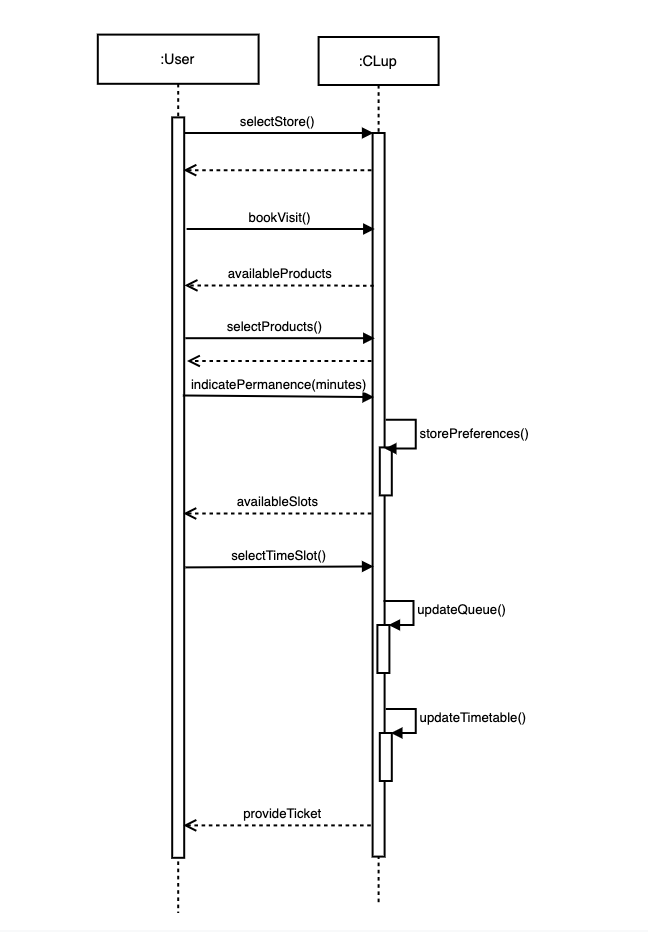
\includegraphics[scale=1.1]{BookAVisit.png}
								\caption{}
								\label{fig:bookavisit_sequencediagram}
							\end{figure}
							\newpage
						
						\item Delete Visit
							\begin{figure}[H]
								\centering
								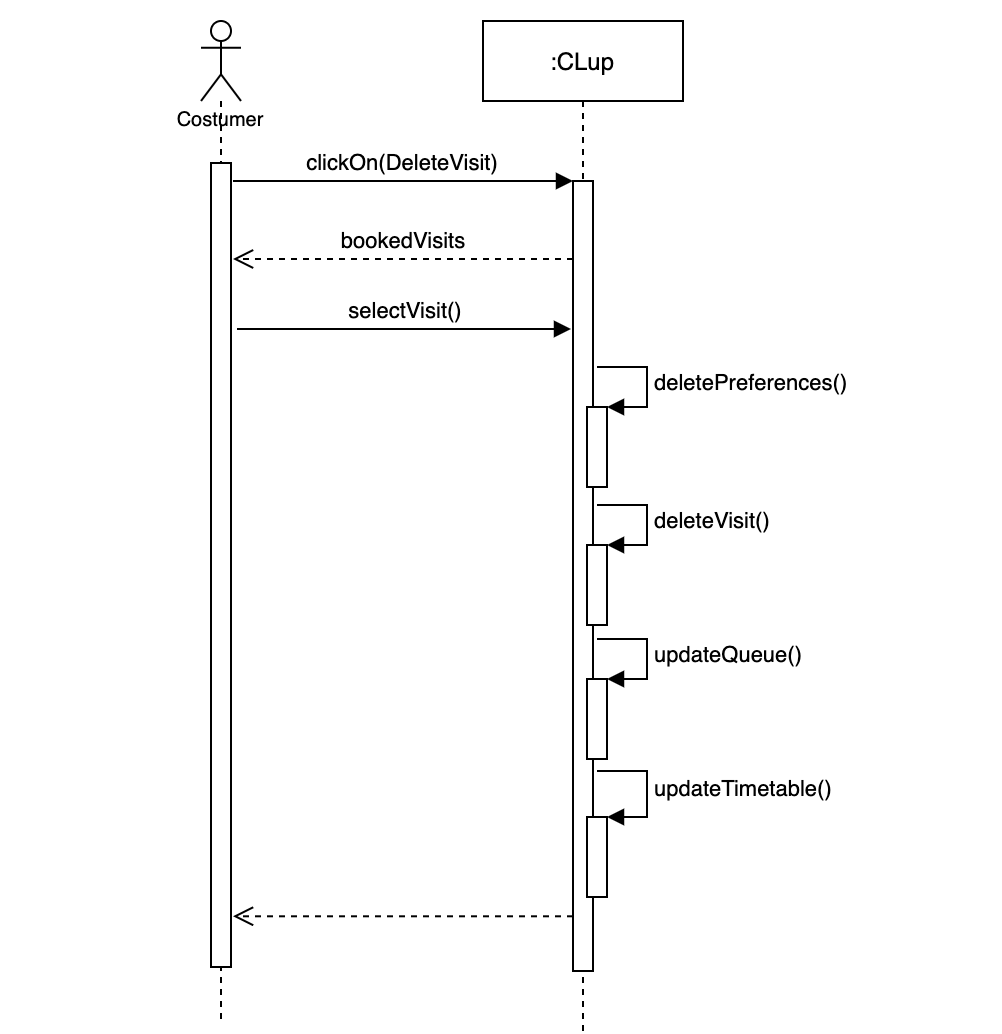
\includegraphics[scale=0.6]{DeleteVisit.png}
								\caption{}
								\label{fig:deletevisit_sequencediagram}
							\end{figure}
							
						\item Physical Lining Up
							\begin{figure}[H]
								\centering
								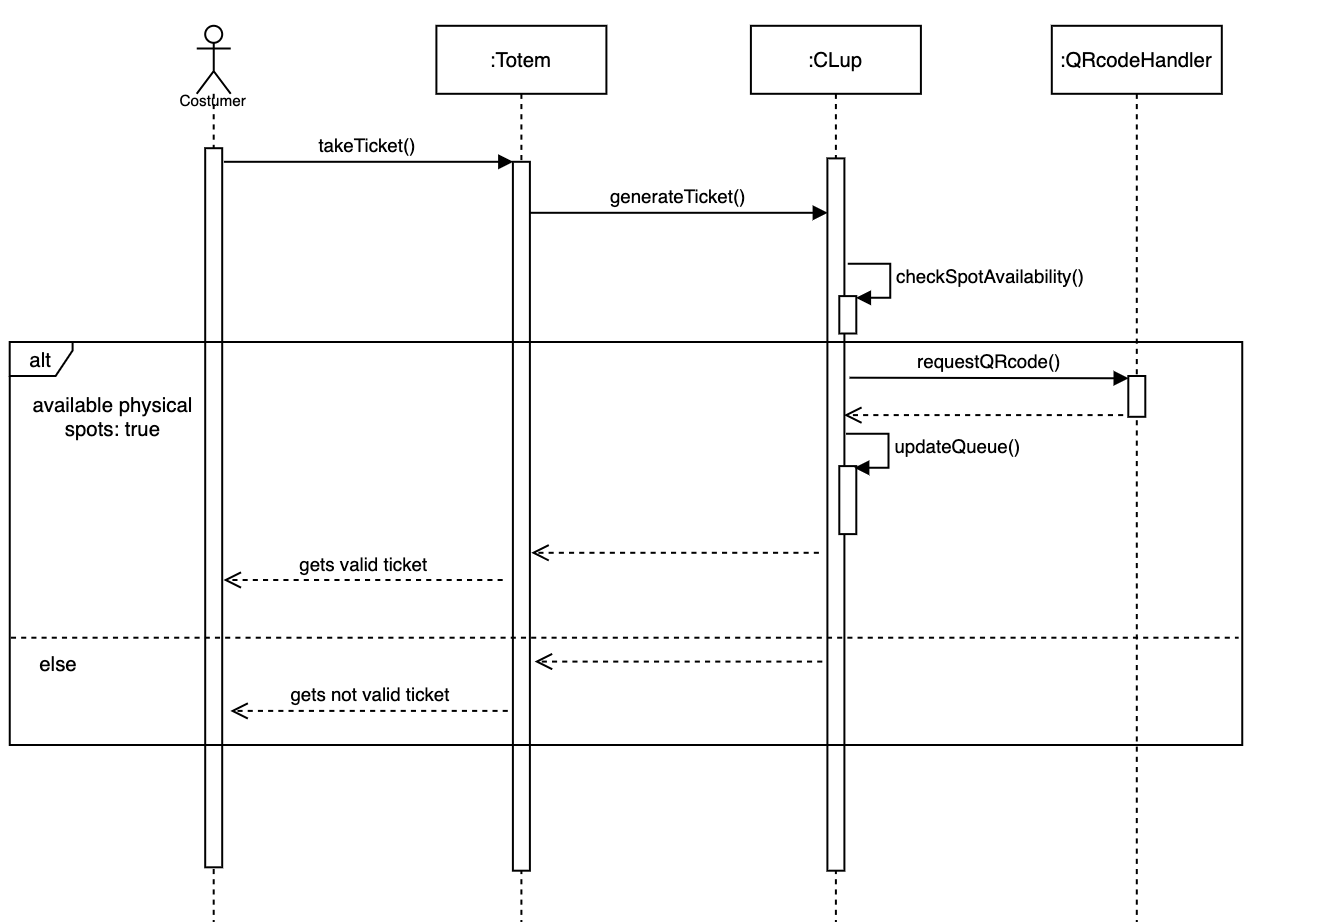
\includegraphics[width=\linewidth]{PhysicalTicket.png}
								\caption{}
								\label{fig:physicalticket_sequencediagram}
							\end{figure}
						
						\item User Enters / Exits the Store
							\begin{figure}[H]
								\centering
								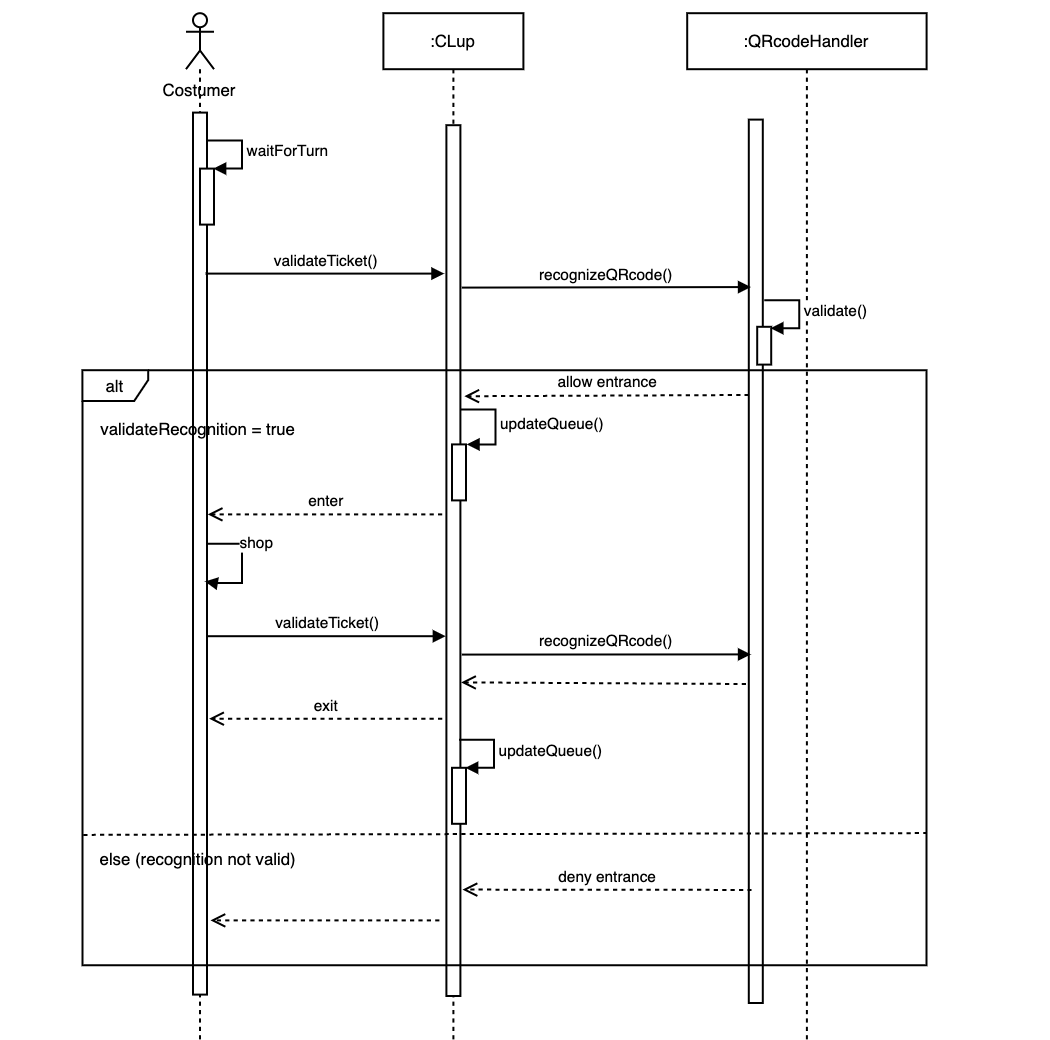
\includegraphics[scale=1.1]{enterexit.png}
								\caption{}
								\label{fig:enterexit_sequencediagram}
							\end{figure}

							
						\item Build Statistics / Preferences
							\begin{figure}[H]
								\centering
								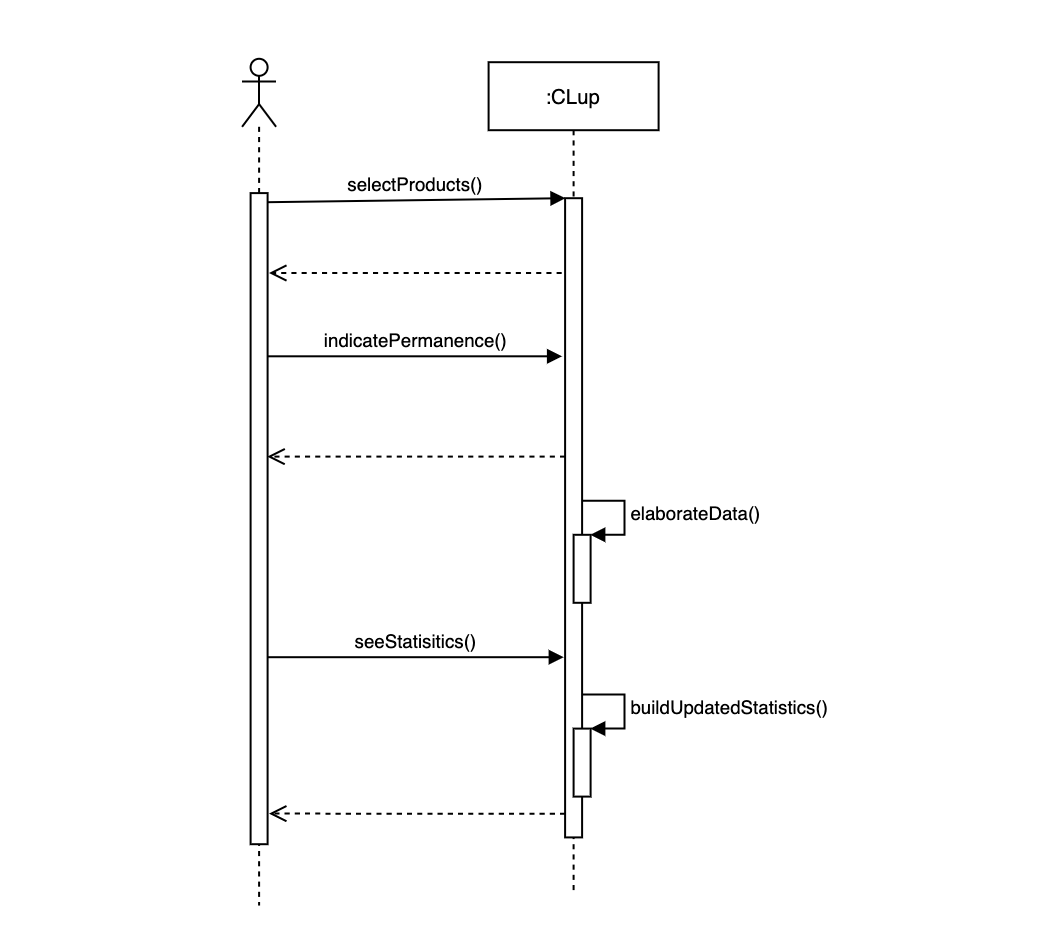
\includegraphics[width=\linewidth]{buildStats.png}
								\caption{}
								\label{fig:buildstats_sequencediagram}
							\end{figure}
						
						\end{enumerate}
		
		\subsection{Performance Requirements}
		
		The system will face a large amount of data. Considering a single store with 50 costumers every hour no problem, but the CLup software must support thousands of registered store and all of them have hundreds of clients every day. Handle this quantity of information brings a meaningful complexity that could cause slowdowns and other problems, therefore, performance should not be underestimated. The system must ensure quick response to every user request, despite the thousands of simultaneous interactions. 
		Then, reliability must be another key feature of the system, therefore there must be less failures as possible.
		
		\subsection{Design Constraints}
		
		\subsubsection{Standard compliance}
		//TODO
		
		\subsubsection{Hardware limitations}
		Every costumer, in order to take full advantage of every system functionality, must be able to face the hardware requirement presented in the \textit{Hardware interfaces} subsection. In fact, the lack of any of them will disable some CLup feature for the user. \\
		For example, if the costumer device isn't equipped with a GPS, the system won't be able to retrieve his position and compute the store reaching time. Therefore, the alert mechanism will be disabled for this user.
		
		\subsubsection{Other constraints}
		//TODO SE CE NE SONO
			

		 
		\subsection{Software System Attributes - Non-Functional Requirements}
			\subsubsection{Reliability and Availability}
			
			The  system should be up at least for the 99,9\% of the time, so the average time between it goes down and then it is recovered (MTTR) should not be higher than 9 hours per year. This also implies that the system should always guarantee that the needed services and functions are satisfied.\\
This high availability of the system needs to be provided because it is related to an emergency situation, and the users should always be able to decide to go shopping when they need (also because in this way they are likely to be distributed during the day). If this condition is not satisfied, there’s the high risk that when the service will be recovered,  all the people would go at the same time to the stores, and the overcrowding problem won’t be avoided anymore.\\
Because we want to ensure this high grade of availability, a system of redundant servers can be considered. However, we can also take into account to have a prepared team that can recover the system as fast as possible when it’s needed, while the users have been notified both when the system is down and when its services are restored and work properly.\\

			\subsubsection{Security}
			
			Passwords of the users and of the managers in the stores need to be protected, so before storing them they need to be correctly encrypted. A similar treatment has to be made also for the preferences pointed out by the users and stored by the system when they are lining up. What’s more,  for what concerns the managers, a periodical update of their password can guarantee a higher protection of the data collected and used by the store. Of course, the system should be protected against intrusion from agent that are not authorized to access it. \\
			
			\subsubsection{Maintainability}
			
			As previously said, the system must be flexible and easy to maintain. For this reason a proper use of design pattern has to be made, as well as a good level of abstraction, so that if the code needs to be extended with new features, everything could be made without any kind of deep code changes. Code must also be well commented and tests on main features of the system should always be working.\\
			
			\subsubsection{Portability}

			The software must run on different platforms, being compatible with the different devices that can be used: for example, managers at the store and users at home could use computers, so the services of the system need to be made usable on Windows OS, Linux OS and MacOS; because of the mobile application, it must be supported a version for Android, iOS and HarmonyOS.\\
			
			\subsubsection{Scalability}

			Everyone will use Clup because of emergency reasons, so the scalability of the system is one of the most important issues to deal with. An high reaction time needs to be reached, so as a consequence it must be set a proper number of processors, devices and memory.\\




		
	\section{Formal analysis using Alloy}
	
	\newpage
	
	\section{Effort spent}
	
	\medskip
	\textbf{\large Antonio Ercolani:} \\ \newline
	\begin{tabular}{|l|c|}
		\hline
		Discussion on the first section &  \textbf{2h} \\ \hline
		\rowcolor[HTML]{DCDCDC} 
		Purpose and Document Structure & \textbf{1,5h} \\ \hline
		Product Functions and User Characteristics & \textbf{3h} \\ \hline
		\rowcolor[HTML]{DCDCDC}
		Discussion on Requirements and Use Cases & \textbf{3h} \\ \hline
		Use cases & \textbf{3h} \\ \hline
		\rowcolor[HTML]{DCDCDC}
		Performance requirements and Design Constraints & \textbf{1h} \\ \hline
	\end{tabular}
	
	
	\textbf{} \newline
	\textbf{} \newline

	\textbf{\large Vittorio Fabris:} \\ \newline
		\begin{tabular}{|l|c|}
			\hline
			Discussion on the first section &  \textbf{2h} \\ \hline
			\rowcolor[HTML]{DCDCDC} 
			Scope & \textbf{3h} \\ \hline
			State Diagrams & \textbf{3h} \\ \hline
			\rowcolor[HTML]{DCDCDC} 
			Discussion on Requirements and Use Cases & \textbf{3h} \\ \hline
		\end{tabular}
		
		

	
	\textbf{\large \\ \\ Riccardo Nannini:} \\ \newline
		\begin{tabular}{|l|c|}
			\hline
			Discussion on the first section &  \textbf{2h} \\ \hline
			\rowcolor[HTML]{DCDCDC} 
			World and Shared Phenomena \& Goals & \textbf{3h} \\ \hline
			Product perspective \& class diagram & \textbf{3h} \\ \hline
			\rowcolor[HTML]{DCDCDC} 
			Discussion on Requirements and Use Cases & \textbf{3h} \\ \hline
			Use Cases \& 3.1 section & \textbf{3h} \\ \hline
		\end{tabular}
	
	\section{References}				
\end{document}
